%%%%%%%%%%%%%%%%%%%%%%%%%%%%%%%%%%%%%%%%%%%%%%%%%%%%%%%%%%%%%%%%%%%%%%%%%%%%%%%%%%%%%%%%%%%%%%%%%%%%%%%%%%%%%%%%%%%%%%%%%%%%%%%%%%%%%%%%%%%%%%%%%%%%%%%%%%%
% This is just an example/guide for you to refer to when submitting manuscripts to Frontiers, it is not mandatory to use Frontiers .cls files nor frontiers.tex  %
% This will only generate the Manuscript, the final article will be typeset by Frontiers after acceptance.
%                                              %
%                                                                                                                                                         %
% When submitting your files, remember to upload this *tex file, the pdf generated with it, the *bib file (if bibliography is not within the *tex) and all the figures.
%%%%%%%%%%%%%%%%%%%%%%%%%%%%%%%%%%%%%%%%%%%%%%%%%%%%%%%%%%%%%%%%%%%%%%%%%%%%%%%%%%%%%%%%%%%%%%%%%%%%%%%%%%%%%%%%%%%%%%%%%%%%%%%%%%%%%%%%%%%%%%%%%%%%%%%%%%%

%%% Version 3.4 Generated 2018/06/15 %%%
%%% You will need to have the following packages installed: datetime, fmtcount, etoolbox, fcprefix, which are normally inlcuded in WinEdt. %%%
%%% In http://www.ctan.org/ you can find the packages and how to install them, if necessary. %%%

\documentclass[utf8]{frontiersSCNS}

%\setcitestyle{square} % for Physics and Applied Mathematics and Statistics articles
\usepackage{url,hyperref,lineno,microtype,subcaption}
\usepackage[onehalfspacing]{setspace}

\linenumbers


% BELOW TAKEN FROM rticles plos template
%
% amsmath package, useful for mathematical formulas
\usepackage{amsmath}
% amssymb package, useful for mathematical symbols
\usepackage{amssymb}

% hyperref package, useful for hyperlinks
\usepackage{hyperref}

% graphicx package, useful for including eps and pdf graphics
% include graphics with the command \includegraphics
\usepackage{graphicx}

% Sweave(-like)
\usepackage{fancyvrb}
\DefineVerbatimEnvironment{Sinput}{Verbatim}{fontshape=sl}
\DefineVerbatimEnvironment{Soutput}{Verbatim}{}
\DefineVerbatimEnvironment{Scode}{Verbatim}{fontshape=sl}
\newenvironment{Schunk}{}{}
\DefineVerbatimEnvironment{Code}{Verbatim}{}
\DefineVerbatimEnvironment{CodeInput}{Verbatim}{fontshape=sl}
\DefineVerbatimEnvironment{CodeOutput}{Verbatim}{}
\newenvironment{CodeChunk}{}{}

% cite package, to clean up citations in the main text. Do not remove.
\usepackage{cite}

\usepackage{color}

\providecommand{\tightlist}{%
  \setlength{\itemsep}{0pt}\setlength{\parskip}{0pt}}

% Below is from frontiers
%
\bibliographystyle{frontiersinSCNS}
% Use doublespacing - comment out for single spacing
%\usepackage{setspace}
%\doublespacing


% Leave a blank line between paragraphs instead of using \\


\def\keyFont{\fontsize{8}{11}\helveticabold }


%% ** EDIT HERE **
%% PLEASE INCLUDE ALL MACROS BELOW

%% END MACROS SECTION

% Pandoc citation processing
\usepackage{booktabs}
\usepackage{longtable}
\usepackage{array}
\usepackage{multirow}
\usepackage{wrapfig}
\usepackage{float}
\usepackage{colortbl}
\usepackage{pdflscape}
\usepackage{tabu}
\usepackage{threeparttable}
\usepackage{threeparttablex}
\usepackage[normalem]{ulem}
\usepackage{makecell}
\usepackage{xcolor}

\usepackage{color}
\usepackage{fancyvrb}
\newcommand{\VerbBar}{|}
\newcommand{\VERB}{\Verb[commandchars=\\\{\}]}
\DefineVerbatimEnvironment{Highlighting}{Verbatim}{commandchars=\\\{\}}
% Add ',fontsize=\small' for more characters per line
\usepackage{framed}
\definecolor{shadecolor}{RGB}{248,248,248}
\newenvironment{Shaded}{\begin{snugshade}}{\end{snugshade}}
\newcommand{\AlertTok}[1]{\textcolor[rgb]{0.94,0.16,0.16}{#1}}
\newcommand{\AnnotationTok}[1]{\textcolor[rgb]{0.56,0.35,0.01}{\textbf{\textit{#1}}}}
\newcommand{\AttributeTok}[1]{\textcolor[rgb]{0.77,0.63,0.00}{#1}}
\newcommand{\BaseNTok}[1]{\textcolor[rgb]{0.00,0.00,0.81}{#1}}
\newcommand{\BuiltInTok}[1]{#1}
\newcommand{\CharTok}[1]{\textcolor[rgb]{0.31,0.60,0.02}{#1}}
\newcommand{\CommentTok}[1]{\textcolor[rgb]{0.56,0.35,0.01}{\textit{#1}}}
\newcommand{\CommentVarTok}[1]{\textcolor[rgb]{0.56,0.35,0.01}{\textbf{\textit{#1}}}}
\newcommand{\ConstantTok}[1]{\textcolor[rgb]{0.00,0.00,0.00}{#1}}
\newcommand{\ControlFlowTok}[1]{\textcolor[rgb]{0.13,0.29,0.53}{\textbf{#1}}}
\newcommand{\DataTypeTok}[1]{\textcolor[rgb]{0.13,0.29,0.53}{#1}}
\newcommand{\DecValTok}[1]{\textcolor[rgb]{0.00,0.00,0.81}{#1}}
\newcommand{\DocumentationTok}[1]{\textcolor[rgb]{0.56,0.35,0.01}{\textbf{\textit{#1}}}}
\newcommand{\ErrorTok}[1]{\textcolor[rgb]{0.64,0.00,0.00}{\textbf{#1}}}
\newcommand{\ExtensionTok}[1]{#1}
\newcommand{\FloatTok}[1]{\textcolor[rgb]{0.00,0.00,0.81}{#1}}
\newcommand{\FunctionTok}[1]{\textcolor[rgb]{0.00,0.00,0.00}{#1}}
\newcommand{\ImportTok}[1]{#1}
\newcommand{\InformationTok}[1]{\textcolor[rgb]{0.56,0.35,0.01}{\textbf{\textit{#1}}}}
\newcommand{\KeywordTok}[1]{\textcolor[rgb]{0.13,0.29,0.53}{\textbf{#1}}}
\newcommand{\NormalTok}[1]{#1}
\newcommand{\OperatorTok}[1]{\textcolor[rgb]{0.81,0.36,0.00}{\textbf{#1}}}
\newcommand{\OtherTok}[1]{\textcolor[rgb]{0.56,0.35,0.01}{#1}}
\newcommand{\PreprocessorTok}[1]{\textcolor[rgb]{0.56,0.35,0.01}{\textit{#1}}}
\newcommand{\RegionMarkerTok}[1]{#1}
\newcommand{\SpecialCharTok}[1]{\textcolor[rgb]{0.00,0.00,0.00}{#1}}
\newcommand{\SpecialStringTok}[1]{\textcolor[rgb]{0.31,0.60,0.02}{#1}}
\newcommand{\StringTok}[1]{\textcolor[rgb]{0.31,0.60,0.02}{#1}}
\newcommand{\VariableTok}[1]{\textcolor[rgb]{0.00,0.00,0.00}{#1}}
\newcommand{\VerbatimStringTok}[1]{\textcolor[rgb]{0.31,0.60,0.02}{#1}}
\newcommand{\WarningTok}[1]{\textcolor[rgb]{0.56,0.35,0.01}{\textbf{\textit{#1}}}}

\def\Authors{
  Samual Smeal\,\textsuperscript{1},
  Anthony Davidson\,\textsuperscript{2},
  Course Lecture (coming)\,\textsuperscript{1,3*}}

\def\Address{

  \textsuperscript{1} School of Biology, ANU, Institution X,  City X,  State XX,  Country X
  
  \textsuperscript{2} Department X, Institution X,  City X,  State XX,  Country X
  }

  
  \def\firstAuthorLast{Smeal {et~al.}}
  
  
  \def\corrAuthor{Course Lecture (coming)}\def\corrAddress{Australian National University\\Civic\\Canberra, ACT, 2061 Australia}\def\corrEmail{\href{mailto:anthony.davidson@anu.edu.au}{\nolinkurl{anthony.davidson@anu.edu.au}}}
  


\begin{document}
\onecolumn
\firstpage{1}

\title[Understanding Simpsons Paradox]{Understanding differences between continuous and discrete distributions
for statistical models in ENVI200+ ANU course}
\author[\firstAuthorLast]{\Authors}
\address{} %This field will be automatically populated
\correspondance{} %This field will be automatically populated

\extraAuth{}% If there are more than 1 corresponding author, comment this line and uncomment the next one.
%\extraAuth{corresponding Author2 \\ Laboratory X2, Institute X2, Department X2, Organization X2, Street X2, City X2 , State XX2 (only USA, Canada and Australia), Zip Code2, X2 Country X2, email2@uni2.edu}


\maketitle

\begin{abstract}

Abstract length and content varies depending on article type. Refer to \url{http://www.frontiersin.org/about/AuthorGuidelines} for abstract requirement and length according to article type.

%All article types: you may provide up to 8 keywords; at least 5 are mandatory.

Understanding the population dynamics of a population can be vital for understanding the projection of these populations to different states of abundance and growth. 

"*Polytelis swainsonii* – Superb Parrot are a non-excavating species and rely on the presence of tree hollows in a given area to make nests. The species are in what is known to be an extinction debt and without the recruitment of new trees amongst the landscape, the superb parrot will be in an expected decline. To increase the chances of incorporating land management practices, key characteristics based on nest selection of the Superb Parrot will be identified using two main methods including single rope climbing techniques and ground based observational methods. I then used this data to find whether tree physiognomy can be used to predict the number of active nests and the presence of hollows. The Study site is based in surrounding Canberra, a key site to mimic a landscape with little to no recruitment of new trees. Highlighting current and future obstacles regarding the management of hollow bearing woodlands seen across most superb parrot nesting populations 
I found that climbing data is more accurate compared to ground-based methods in counting tree hollows and tree hollow nests. On average climbing data increased the ground count by 32%  and nests found in this method found 2.1x the amount of ground based methods. 
 (insert data here maybe) Super  parrots prefer a tree DBH  on average 114cm to hollows without a nest 102cm. 
 
Using a double sampling technique paired with a critical ratio, climbing and ground based results in ongoing studies can further contribute to this area of study by replicating the process used in this report.  Citizen science projects can benefit in the future by focusing on the key indicators highlighted and thus increase the effectiveness across future measurements. 
citizen science projects can measurements can be calibrated using double sampling techniques to correct data derived from future citizen science projects, savings costs overall and improving management studies by increasing the observability of simple measurements such as tree DBH"

\tiny
 \keyFont{ \section{Keywords:} Biology, Statistics, Ecology, Simpsons paradox} 

\end{abstract}

\hypertarget{introduction}{%
\section*{Introduction}\label{introduction}}
\addcontentsline{toc}{section}{Introduction}

Individual biases in the scientific endenvour is a fundamental task of
any researcher. This publication links the open-sources tools and
templates that allow to for the production of typed set articles.

Here is an example of a simple journal submission template for the
journal ``Frontiers in Science'' and the association information needed
(LastName1 et al., 2013). As demonstrated in OtherAuthor and Coauthor
(2012), citations can also be automatically reference. Multiple
references are separated by semicolons (LastName1 et al., 2013; Author4
and Author5, 2013a). I have used this template to generate a simple
description and information about a important issue when comparing means
of two samples.

Simpsons paradox (Author4 and Author5, 2013b) is a phenomenon where the
true relationship between between two groups is missed due to a
underlying, interactions between an unmeasured variable and the two
groups being investigated.

(Simpson, 1951)

This can occur and not be know but often it happens that later research
can identify these paradoxical relationships with additional data. The
study set up for this experiment has the potential for this to occur,
particularly because of the modification and manipulation of the
original data.

\hypertarget{methods}{%
\section*{Methods}\label{methods}}
\addcontentsline{toc}{section}{Methods}

``Methods Study area and species The data collected was from North
Canberra in two sites, the outskirts of Throsby just outside of
mulligans flat reserve -35.172074, 149.165799 and south west of
Belconnen -35.241217, 149.004370 where the superb parrot is known to
breed in colonies on the outskirts of Canberra. The two study sites are
roughly 15km apart on either side of suburban Canberra and can be
considered independent of each other with localised climate history and
also dependent on preference due to the ability of the superb parrots
metapopulation not being limited to the distance between the study
sites. The study sites are heavily grazed open woodlands used for mostly
cattle. The trees are mostly all aged hollow bearing little to no
recruitment of young trees sue to the current land uses. For this study
sites measurements were derived by only two tree species, Eucalytpus
blakleyi (Blakely's red gum) and Eucalyptus rosii (Scribbly Gum)''

\hypertarget{continuous-variables}{%
\subsubsection{Continuous variables}\label{continuous-variables}}

A continuous variable is estimated with a mean and SD and contains
values that include all real numbers. The first data set has the
following arrangement of continuous and discrete variables.

\begin{Shaded}
\begin{Highlighting}[]
\CommentTok{#data}
\NormalTok{dat_hol <-}\StringTok{ }\KeywordTok{read_xlsx}\NormalTok{(here}\OperatorTok{::}\KeywordTok{here}\NormalTok{(}\StringTok{"SamsRepo/data/hollow_data_wrangled.xlsx"}\NormalTok{),}\DataTypeTok{sheet =} \DecValTok{1}\NormalTok{) }\OperatorTok
\KeywordTok{mutate}\NormalTok{(}\DataTypeTok{BirdPresence =} \KeywordTok{factor}\NormalTok{(birdPresent),}
\DataTypeTok{spp =} \KeywordTok{factor}\NormalTok{(}\StringTok{'tree species'}\NormalTok{))}

\NormalTok{kableExtra}\OperatorTok{::}\KeywordTok{kable}\NormalTok{(}\KeywordTok{glimpse}\NormalTok{(}\KeywordTok{head}\NormalTok{(dat_hol)))}
\end{Highlighting}
\end{Shaded}

\begin{verbatim}
## Rows: 6
## Columns: 9
## $ birdPresent                                  <chr> "no", "no", "no", "no", "~
## $ `number of entrance holes per hollow`        <dbl> 1, 1, 2, 2, 1, 1
## $ `minimum entrance diameter (cm)`             <dbl> 6, 9, 10, 13, 4, 4
## $ `floor diameter (cm)`                        <dbl> 8, 9, 10, 26, 5, 8
## $ `depth of hollow (cm)`                       <dbl> 61, 19, 72, 70, 35, 59
## $ `diameter of the stem the hollow is in (cm)` <dbl> 17, 15, 18, 43, 91, 16
## $ `tree species`                               <chr> "blakelyi", "blakelyi", "~
## $ BirdPresence                                 <fct> no, no, no, no, no, no
## $ spp                                          <fct> tree species, tree specie~
\end{verbatim}

\begin{tabular}{l|r|r|r|r|r|l|l|l}
\hline
birdPresent & number of entrance holes per hollow & minimum entrance diameter (cm) & floor diameter (cm) & depth of hollow (cm) & diameter of the stem the hollow is in (cm) & tree species & BirdPresence & spp\\
\hline
no & 1 & 6 & 8 & 61 & 17 & blakelyi & no & tree species\\
\hline
no & 1 & 9 & 9 & 19 & 15 & blakelyi & no & tree species\\
\hline
no & 2 & 10 & 10 & 72 & 18 & blakelyi & no & tree species\\
\hline
no & 2 & 13 & 26 & 70 & 43 & blakelyi & no & tree species\\
\hline
no & 1 & 4 & 5 & 35 & 91 & blakelyi & no & tree species\\
\hline
no & 1 & 4 & 8 & 59 & 16 & blakelyi & no & tree species\\
\hline
\end{tabular}

\begin{Shaded}
\begin{Highlighting}[]
\NormalTok{varnames_hol <-}\StringTok{ }\KeywordTok{read_xlsx}\NormalTok{(here}\OperatorTok{::}\KeywordTok{here}\NormalTok{(}\StringTok{"SamsRepo/data/hollow_data_wrangled.xlsx"}\NormalTok{),}\DataTypeTok{sheet =} \DecValTok{2}\NormalTok{)}

\KeywordTok{names}\NormalTok{(dat_hol)[}\DecValTok{1}\OperatorTok{:}\DecValTok{7}\NormalTok{] <-}\StringTok{ }\NormalTok{varnames_hol}\OperatorTok{$}\NormalTok{shortname}

\NormalTok{dat_hol <-}\StringTok{ }\NormalTok{dat_hol[,}\DecValTok{1}\OperatorTok{:}\DecValTok{7}\NormalTok{]}
  
\NormalTok{dat_hol }\OperatorTok\StringTok{ }
\StringTok{  }\KeywordTok{ggplot}\NormalTok{(}\DataTypeTok{mapping =} \KeywordTok{aes}\NormalTok{(}\DataTypeTok{x =}\NormalTok{ hollows, }\DataTypeTok{col =}\NormalTok{ birdpresent, }\DataTypeTok{fill =}\NormalTok{ spp)) }\OperatorTok{+}
\StringTok{  }\CommentTok{# geom_histogram(position = "dodge", stat = "count") +}
\StringTok{  }\KeywordTok{geom_density}\NormalTok{() }\OperatorTok{+}\StringTok{ }
\StringTok{  }\KeywordTok{facet_grid}\NormalTok{(}\StringTok{"floorDia"}\OperatorTok{~}\NormalTok{spp) }\OperatorTok{+}\StringTok{ }
\StringTok{  }\KeywordTok{coord_cartesian}\NormalTok{() }\OperatorTok{+}\StringTok{ }
\StringTok{  }\KeywordTok{ggtitle}\NormalTok{(}\StringTok{"Density of the presence of active and non active nest hollows compared to number of hollows"}\NormalTok{)}
\end{Highlighting}
\end{Shaded}

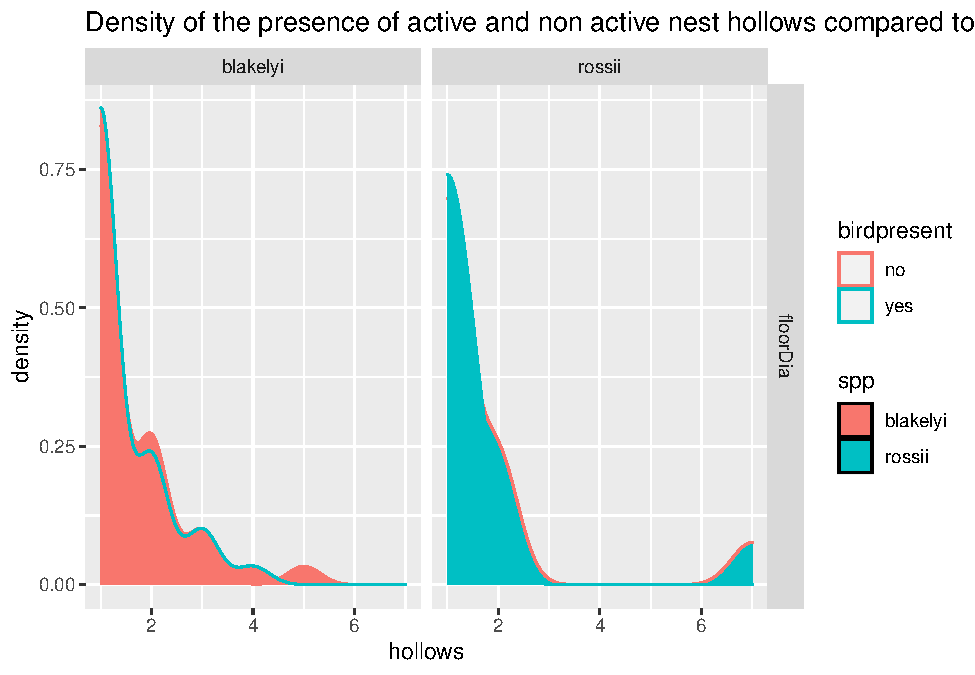
\includegraphics{demoReport_files/figure-latex/unnamed-chunk-1-1.pdf}

\hypertarget{floor-diameter}{%
\paragraph{Floor diameter}\label{floor-diameter}}

\begin{Shaded}
\begin{Highlighting}[]
\KeywordTok{names}\NormalTok{(dat_hol)}
\end{Highlighting}
\end{Shaded}

\begin{verbatim}
## [1] "birdpresent"    "hollows"        "minDiaEntrance" "floorDia"      
## [5] "depthCm"        "diaCm"          "spp"
\end{verbatim}

\begin{Shaded}
\begin{Highlighting}[]
\NormalTok{dat_hol }\OperatorTok\StringTok{ }
\StringTok{  }\KeywordTok{ggplot}\NormalTok{(}\DataTypeTok{mapping =} \KeywordTok{aes}\NormalTok{(}\DataTypeTok{x =}\NormalTok{ minDiaEntrance, }\DataTypeTok{fill =}\NormalTok{ birdpresent)) }\OperatorTok{+}
\StringTok{  }\CommentTok{# geom_histogram(position = "dodge", stat = "count") +}
\StringTok{  }\KeywordTok{geom_density}\NormalTok{(}\DataTypeTok{bins =} \DecValTok{100}\NormalTok{) }\OperatorTok{+}\StringTok{ }
\StringTok{  }\KeywordTok{facet_grid}\NormalTok{(spp}\OperatorTok{~}\StringTok{"floorDia"}\NormalTok{) }\OperatorTok{+}\StringTok{ }\CommentTok{#}
\StringTok{  }\KeywordTok{coord_cartesian}\NormalTok{() }\OperatorTok{+}\StringTok{ }
\StringTok{  }\KeywordTok{ggtitle}\NormalTok{(}\StringTok{"Density of the presence of active and non active nest hollows compared to number of hollows"}\NormalTok{)}
\end{Highlighting}
\end{Shaded}

\begin{verbatim}
## Warning: Ignoring unknown parameters: bins
\end{verbatim}

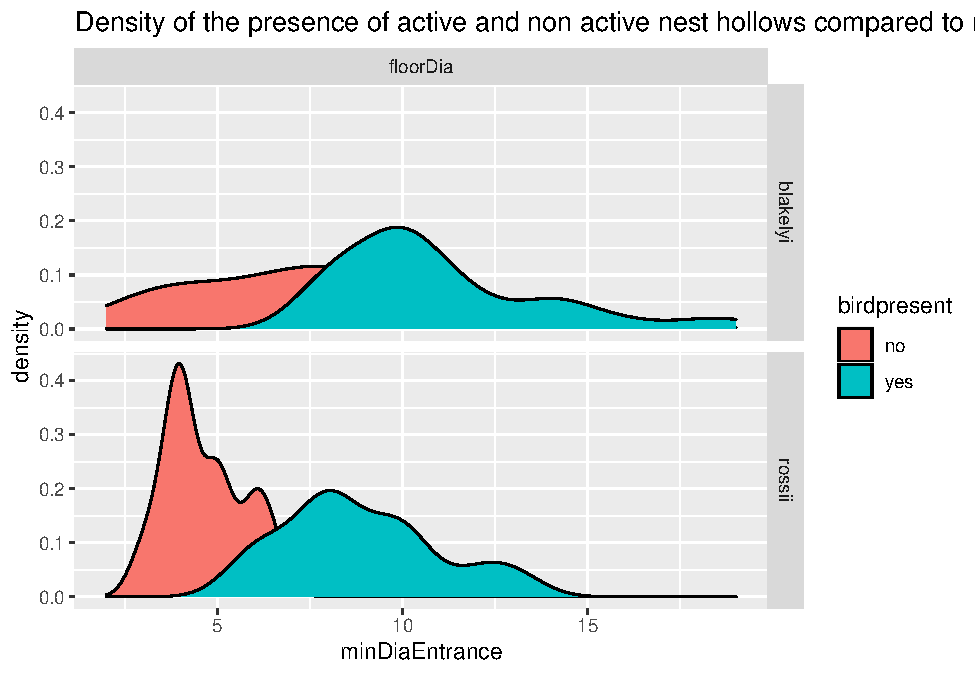
\includegraphics{demoReport_files/figure-latex/unnamed-chunk-2-1.pdf}

\hypertarget{normal}{%
\paragraph{Normal}\label{normal}}

\begin{Shaded}
\begin{Highlighting}[]
\KeywordTok{names}\NormalTok{(dat)}
\end{Highlighting}
\end{Shaded}

\begin{verbatim}
## [1] "BirdPresence"    "treeDiameter"    "healthScale"     "hollowNumber"   
## [5] "hollowEntrances" "spp"
\end{verbatim}

\begin{Shaded}
\begin{Highlighting}[]
\KeywordTok{glimpse}\NormalTok{(dat)}
\end{Highlighting}
\end{Shaded}

\begin{verbatim}
## Rows: 50
## Columns: 6
## $ BirdPresence    <fct> no, no, no, no, no, no, no, no, no, no, no, no, no, no~
## $ treeDiameter    <dbl> 125, 100, 106, 136, 70, 113, 95, 83, 67, 48, 96, 99, 1~
## $ healthScale     <dbl> 4, 2, 3, 4, 4, 4, 2, 3, 2, 4, 2, 4, 1, 1, 2, 3, 3, 3, ~
## $ hollowNumber    <dbl> 5, 1, 11, 9, 2, 13, 4, 4, 2, 0, 3, 1, 3, 18, 6, 5, 0, ~
## $ hollowEntrances <dbl> 3, 2, 3, 7, 2, 14, 3, 2, 1, 1, 0, 3, 3, 9, 7, 3, 2, 1,~
## $ spp             <fct> blakelyi, blakelyi, blakelyi, blakelyi, blakelyi, blak~
\end{verbatim}

\begin{Shaded}
\begin{Highlighting}[]
\NormalTok{dat1 <-}\StringTok{ }\NormalTok{dat[,}\DecValTok{2}\NormalTok{,}\DecValTok{5}\NormalTok{]}
\CommentTok{# plot(lm(select(dat, treeDiameter, healthScale), subset = dat$BirdPresence))}

\NormalTok{varNames <-}\StringTok{ }\KeywordTok{names}\NormalTok{(dat)}
\NormalTok{varLength <-}\StringTok{ }\KeywordTok{length}\NormalTok{(}\KeywordTok{names}\NormalTok{(dat))}
\CommentTok{# for(i in 1:varLength) \{}
\CommentTok{#   i = 2}
\CommentTok{#   mod <- lm(select(dat, varNames[i]))}
\CommentTok{#   }
\CommentTok{#   ggplot(dat) + }
\CommentTok{#     geom_histogram(aes(x = dat$varNames[i]), stat = "count")}
\CommentTok{# \}}
\end{Highlighting}
\end{Shaded}

\begin{itemize}
\tightlist
\item
  Tree Diameter
\end{itemize}

\begin{Shaded}
\begin{Highlighting}[]
\NormalTok{dat }\OperatorTok\StringTok{ }
\StringTok{  }\KeywordTok{ggplot}\NormalTok{(}\DataTypeTok{mapping =} \KeywordTok{aes}\NormalTok{(healthScale, }\DataTypeTok{fill =}\NormalTok{ BirdPresence)) }\OperatorTok{+}
\StringTok{  }\KeywordTok{geom_histogram}\NormalTok{(}\DataTypeTok{position =} \StringTok{"dodge"}\NormalTok{) }\OperatorTok{+}
\StringTok{  }\KeywordTok{geom_density}\NormalTok{(}\DataTypeTok{stat =} \StringTok{"count"}\NormalTok{) }\OperatorTok{+}\StringTok{ }
\StringTok{  }\KeywordTok{facet_grid}\NormalTok{(BirdPresence}\OperatorTok{~}\NormalTok{spp) }\OperatorTok{+}\StringTok{ }
\StringTok{  }\KeywordTok{coord_cartesian}\NormalTok{()}
\end{Highlighting}
\end{Shaded}

\begin{verbatim}
## `stat_bin()` using `bins = 30`. Pick better value with `binwidth`.
\end{verbatim}

\begin{center}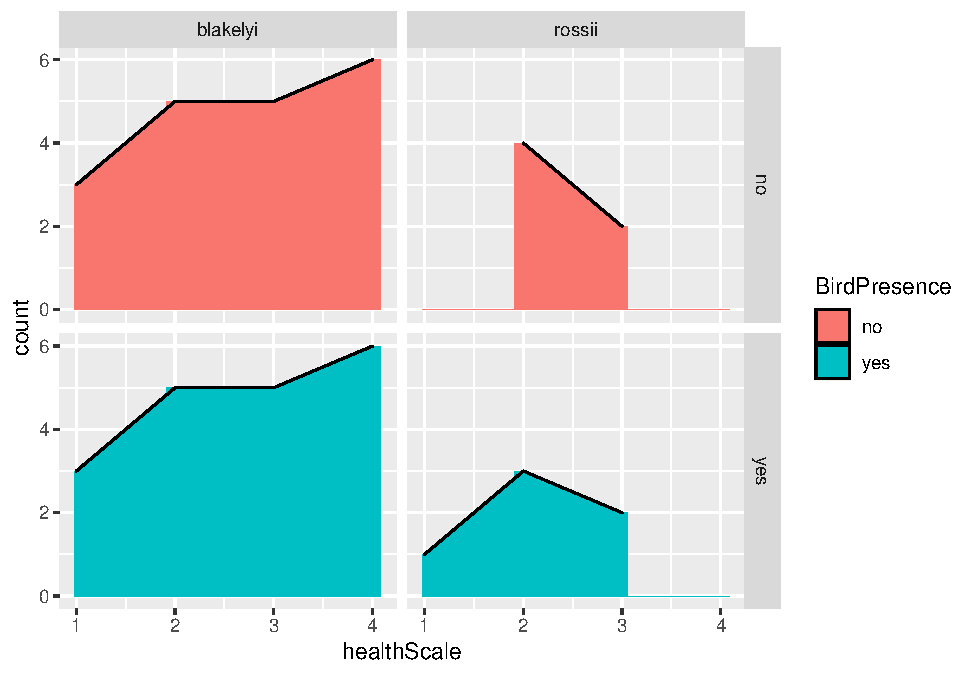
\includegraphics{demoReport_files/figure-latex/unnamed-chunk-4-1} \end{center}

\begin{Shaded}
\begin{Highlighting}[]
\CommentTok{#random health scale?}
\KeywordTok{names}\NormalTok{(dat)}

\NormalTok{rand_scale <-}\StringTok{ }\KeywordTok{filter}\NormalTok{(dat, BirdPresence }\OperatorTok{==}\StringTok{ "no"}\NormalTok{)}


\NormalTok{tallyCounts <-}\StringTok{ }\NormalTok{dat }\OperatorTok
\StringTok{                }\KeywordTok{group_by}\NormalTok{(BirdPresence) }\OperatorTok
\StringTok{                  }\KeywordTok{summarise}\NormalTok{(}\DataTypeTok{treeDiameter =} \KeywordTok{mean}\NormalTok{(treeDiameter),}
                            \DataTypeTok{healthScale =} \KeywordTok{mean}\NormalTok{(healthScale),}
                            \DataTypeTok{hollowEntrances =} \KeywordTok{mean}\NormalTok{(hollowEntrances),}
                            \DataTypeTok{hollowNumber =} \KeywordTok{mean}\NormalTok{(hollowNumber),}
                            \DataTypeTok{Random =} \KeywordTok{mean}\NormalTok{(}\KeywordTok{as.numeric}\NormalTok{(BirdPresence)), }
                            \DataTypeTok{spp =} \KeywordTok{mean}\NormalTok{(}\KeywordTok{as.numeric}\NormalTok{(spp)))}

\NormalTok{tallyCounts}

\NormalTok{y <-}\StringTok{ }\NormalTok{dat}\OperatorTok{$}\NormalTok{BirdPresence}
\NormalTok{x <-}\StringTok{ }\NormalTok{dat}\OperatorTok{$}\NormalTok{healthScale}

\NormalTok{datNull <-}\StringTok{ }\KeywordTok{data.frame}\NormalTok{(y,x)}
\CommentTok{#anova in R}
\CommentTok{#is just glm then avo of output}

\NormalTok{mod <-}\StringTok{ }\KeywordTok{glm}\NormalTok{(y }\OperatorTok{~}\NormalTok{x, }\DataTypeTok{data =}\NormalTok{ datNull, }\DataTypeTok{family =} \StringTok{"binomial"}\NormalTok{)}
\KeywordTok{summary}\NormalTok{(mod)}
\NormalTok{anovaR <-}\StringTok{ }\KeywordTok{anova}\NormalTok{(mod)}

\NormalTok{health_scale}
\end{Highlighting}
\end{Shaded}

\hypertarget{poisson}{%
\paragraph{Poisson}\label{poisson}}

\begin{itemize}
\tightlist
\item
  hollowNumber
\item
  hollowEntrances
\end{itemize}

\begin{Shaded}
\begin{Highlighting}[]
\NormalTok{poisRand10 <-}\StringTok{ }\KeywordTok{rpois}\NormalTok{(}\DecValTok{10}\NormalTok{, }\FloatTok{0.5}\NormalTok{) }\CommentTok{#lambda is growth rate here}
\KeywordTok{plot}\NormalTok{(}\KeywordTok{density}\NormalTok{(poisRand10))}

\NormalTok{poisRand20 <-}\StringTok{ }\KeywordTok{rpois}\NormalTok{(}\DecValTok{20}\NormalTok{, }\FloatTok{0.5}\NormalTok{) }\CommentTok{#lambda is growth rate here}
\KeywordTok{plot}\NormalTok{(}\KeywordTok{density}\NormalTok{(poisRand10))}
\end{Highlighting}
\end{Shaded}

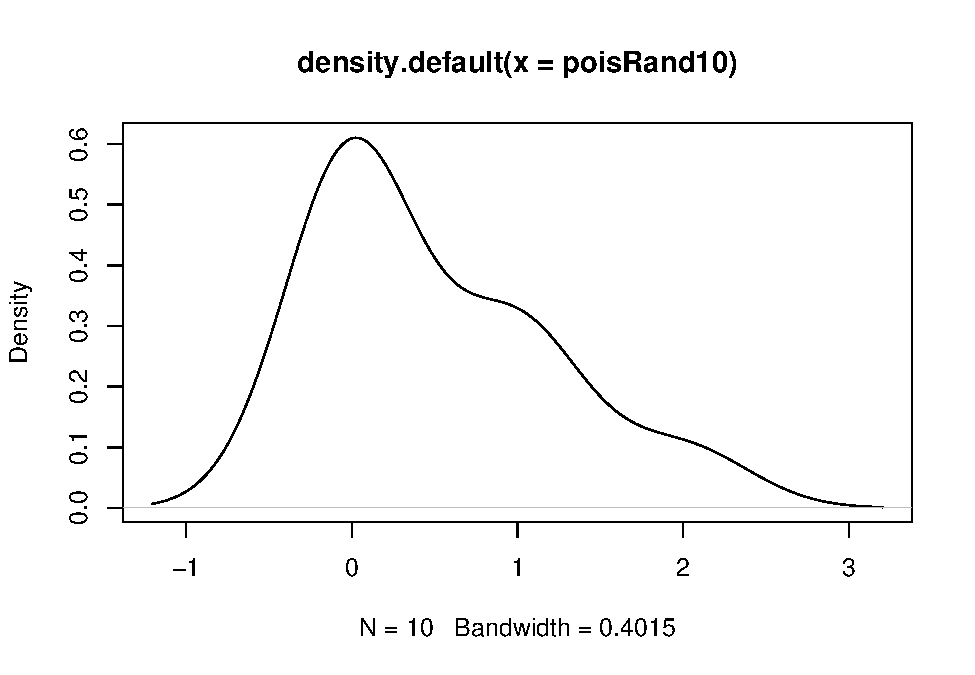
\includegraphics{demoReport_files/figure-latex/unnamed-chunk-6-1.pdf}

\begin{Shaded}
\begin{Highlighting}[]
\NormalTok{poisRand30 <-}\StringTok{ }\KeywordTok{rpois}\NormalTok{(}\DecValTok{30}\NormalTok{, }\FloatTok{0.5}\NormalTok{) }\CommentTok{#lambda is growth rate here}
\KeywordTok{plot}\NormalTok{(}\KeywordTok{density}\NormalTok{(poisRand10))}

\NormalTok{poisRand100 <-}\StringTok{ }\KeywordTok{rpois}\NormalTok{(}\DecValTok{100}\NormalTok{, }\FloatTok{0.5}\NormalTok{) }\CommentTok{#lambda is growth rate here}
\KeywordTok{plot}\NormalTok{(}\KeywordTok{density}\NormalTok{(poisRand100))}
\end{Highlighting}
\end{Shaded}

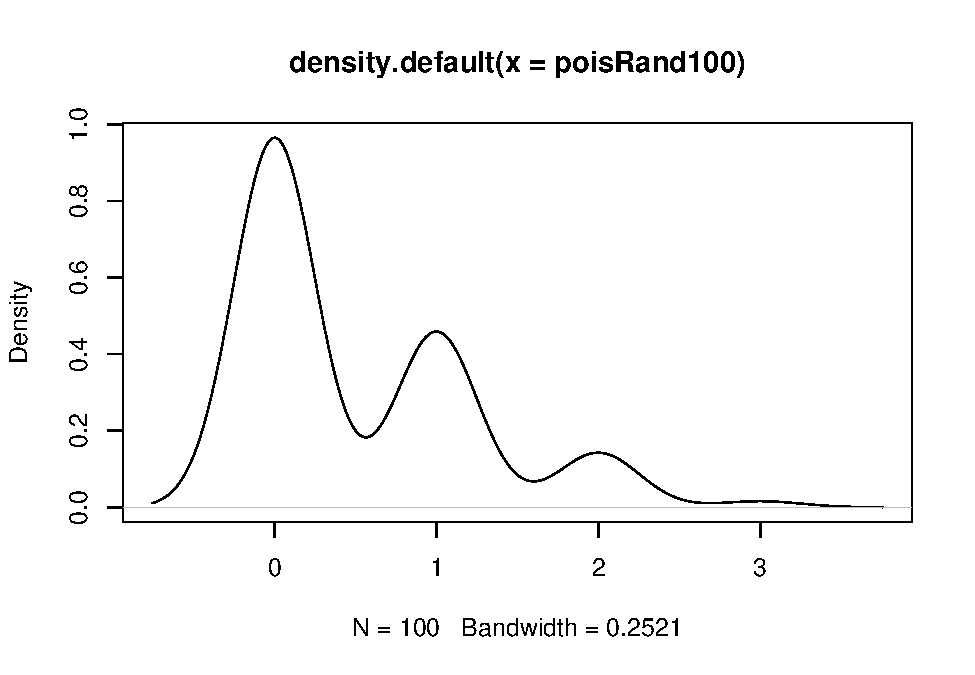
\includegraphics{demoReport_files/figure-latex/unnamed-chunk-6-2.pdf}

\hypertarget{discrete}{%
\paragraph{Discrete}\label{discrete}}

\begin{itemize}
\tightlist
\item
  BirdPresence
\item
  spp
\end{itemize}

\begin{Shaded}
\begin{Highlighting}[]
\CommentTok{# DT::datatable(dat)}
\NormalTok{kableExtra}\OperatorTok{::}\KeywordTok{kable}\NormalTok{(}\KeywordTok{head}\NormalTok{(dat))}
\end{Highlighting}
\end{Shaded}

\begin{tabular}{l|r|r|r|r|l}
\hline
BirdPresence & treeDiameter & healthScale & hollowNumber & hollowEntrances & spp\\
\hline
no & 125 & 4 & 5 & 3 & blakelyi\\
\hline
no & 100 & 2 & 1 & 2 & blakelyi\\
\hline
no & 106 & 3 & 11 & 3 & blakelyi\\
\hline
no & 136 & 4 & 9 & 7 & blakelyi\\
\hline
no & 70 & 4 & 2 & 2 & blakelyi\\
\hline
no & 113 & 4 & 13 & 14 & blakelyi\\
\hline
\end{tabular}

\hypertarget{results}{%
\section*{Results}\label{results}}
\addcontentsline{toc}{section}{Results}

\begin{Shaded}
\begin{Highlighting}[]
\NormalTok{p1 <-}\StringTok{ }\NormalTok{dat }\OperatorTok\StringTok{ }
\StringTok{  }\KeywordTok{ggplot}\NormalTok{(}\DataTypeTok{mapping =} \KeywordTok{aes}\NormalTok{(treeDiameter, }\DataTypeTok{group =}\NormalTok{ BirdPresence)) }\OperatorTok{+}
\StringTok{  }\KeywordTok{geom_density}\NormalTok{() }\OperatorTok{+}
\StringTok{  }\KeywordTok{facet_grid}\NormalTok{(spp}\OperatorTok{~}\NormalTok{BirdPresence)}

\NormalTok{p2 <-}\StringTok{ }\NormalTok{dat }\OperatorTok\StringTok{ }
\StringTok{  }\KeywordTok{ggplot}\NormalTok{(}\DataTypeTok{mapping =} \KeywordTok{aes}\NormalTok{(spp)) }\OperatorTok{+}
\StringTok{  }\KeywordTok{geom_histogram}\NormalTok{(}\DataTypeTok{stat =} \StringTok{"count"}\NormalTok{) }\OperatorTok{+}
\StringTok{  }\KeywordTok{coord_cartesian}\NormalTok{()}
\end{Highlighting}
\end{Shaded}

\begin{verbatim}
## Warning: Ignoring unknown parameters: binwidth, bins, pad
\end{verbatim}

\begin{Shaded}
\begin{Highlighting}[]
\NormalTok{p3 <-}\StringTok{ }\NormalTok{dat }\OperatorTok\StringTok{ }
\StringTok{  }\KeywordTok{ggplot}\NormalTok{(}\DataTypeTok{mapping =} \KeywordTok{aes}\NormalTok{(BirdPresence)) }\OperatorTok{+}
\StringTok{  }\KeywordTok{geom_bar}\NormalTok{() }\OperatorTok{+}
\StringTok{  }\KeywordTok{coord_flip}\NormalTok{()}

\NormalTok{gridExtra}\OperatorTok{::}\KeywordTok{grid.arrange}\NormalTok{(p1,p2,p3)}
\end{Highlighting}
\end{Shaded}

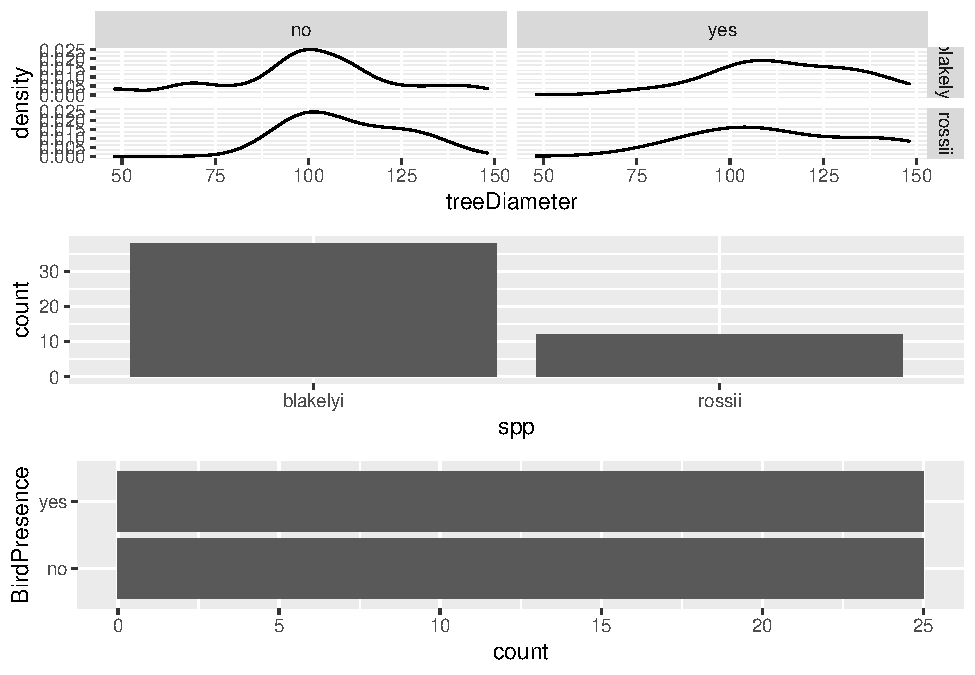
\includegraphics{demoReport_files/figure-latex/unnamed-chunk-8-1.pdf}

\begin{Shaded}
\begin{Highlighting}[]
\CommentTok{# barplot_test <- plot(x = dat$healthScale, y = dat$BirdPresence)}
\CommentTok{# str(dat$BirdPresence)}
\end{Highlighting}
\end{Shaded}

\hypertarget{hollow-data}{%
\subsection*{Hollow data}\label{hollow-data}}
\addcontentsline{toc}{subsection}{Hollow data}

coming???

\begin{Shaded}
\begin{Highlighting}[]
\CommentTok{#balanced hollow}
\NormalTok{dat_holl <-}\StringTok{ }\KeywordTok{read_xlsx}\NormalTok{(here}\OperatorTok{::}\KeywordTok{here}\NormalTok{(}\StringTok{"SamsRepo/data/hollow_data_wrangled.xlsx"}\NormalTok{),}\DataTypeTok{sheet =} \DecValTok{1}\NormalTok{)}
\NormalTok{varnames_holl <-}\StringTok{ }\KeywordTok{read_xlsx}\NormalTok{(here}\OperatorTok{::}\KeywordTok{here}\NormalTok{(}\StringTok{"SamsRepo/data/hollow_data_wrangled.xlsx"}\NormalTok{),}\DataTypeTok{sheet =} \DecValTok{2}\NormalTok{)}
\end{Highlighting}
\end{Shaded}

Frontiers requires figures to be submitted individually, in the same
order as they are referred to in the manuscript. Figures will then be
automatically embedded at the bottom of the submitted manuscript. Kindly
ensure that each table and figure is mentioned in the text and in
numerical order. Permission must be obtained for use of copyrighted
material from other sources (including the web). Please note that it is
compulsory to follow figure instructions. Figures which are not
according to the guidelines will cause substantial delay during the
production process.

\hypertarget{discussion}{%
\section{Discussion}\label{discussion}}

The results of this publication highlight the ability for any
undergraduate course to include the relevent documentation for the
submission of research articles from written text from a word document
from an RMarkdown veriation of this information.

\hypertarget{disclosureconflict-of-interest-statement}{%
\section*{Disclosure/Conflict-of-Interest
Statement}\label{disclosureconflict-of-interest-statement}}
\addcontentsline{toc}{section}{Disclosure/Conflict-of-Interest
Statement}

The authors declare that the research was conducted in the absence of
any commercial or financial relationships that could be construed as a
potential conflict of interest.

\hypertarget{author-contributions}{%
\section*{Author Contributions}\label{author-contributions}}
\addcontentsline{toc}{section}{Author Contributions}

The statement about the authors and contributors can be up to several
sentences long, describing the tasks of individual authors referred to
by their initials and should be included at the end of the manuscript
before the References section.

\hypertarget{acknowledgments}{%
\section*{Acknowledgments}\label{acknowledgments}}
\addcontentsline{toc}{section}{Acknowledgments}

Funding:

\hypertarget{supplemental-data}{%
\section{Supplemental Data}\label{supplemental-data}}

Supplementary Material should be uploaded separately on submission, if
there are Supplementary Figures, please include the caption in the same
file as the figure. LaTeX Supplementary Material templates can be found
in the Frontiers LaTeX folder

\hypertarget{references}{%
\section{References}\label{references}}

A reference list should be automatically created here. However it won't.
Pandoc will place the list of references at the end of the document
instead. There are no convenient solution for now to force Pandoc to do
otherwise. The easiest way to get around this problem is to edit the
LaTeX file created by Pandoc before compiling it again using the
traditional LaTeX commands.

\hypertarget{figures}{%
\section*{Figures}\label{figures}}
\addcontentsline{toc}{section}{Figures}

\hypertarget{refs}{}
\leavevmode\hypertarget{ref-Neurobot2013}{}%
Author4, N., and Author5, N. (2013a). Title of the article.
\emph{Frontiers in Neurorobotics} 7.
doi:\href{https://doi.org/10.3389/fnbot.2013.56789}{10.3389/fnbot.2013.56789}.

\leavevmode\hypertarget{ref-simpsonlink2021}{}%
Author4, N., and Author5, N. (2013b). Title of the article.
\emph{Frontiers in Neurorobotics} 7.
doi:\href{https://doi.org/10.3389/fnbot.2013.56789}{10.3389/fnbot.2013.56789}.

\leavevmode\hypertarget{ref-Neuro2013}{}%
LastName1, A., LastName2, A., and LastName2, A. (2013). Article title.
\emph{Frontiers in Neuroscience} 30, 10127--10134.
doi:\href{https://doi.org/10.3389/fnins.2013.12345}{10.3389/fnins.2013.12345}.

\leavevmode\hypertarget{ref-Gene2012}{}%
OtherAuthor, N., and Coauthor, N. S. (2012). Article title.
\emph{Frontiers in Genetics} 30, 16417--16418.
doi:\href{https://doi.org/10.3389/fgene.2012.54321}{10.3389/fgene.2012.54321}.

\leavevmode\hypertarget{ref-simpson1951interpretation}{}%
Simpson, E. H. (1951). The interpretation of interaction in contingency
tables. \emph{Journal of the Royal Statistical Society: Series B
(Methodological)} 13, 238--241.

\end{document}
